\documentclass[a4paper]{article}
\usepackage{a4wide} 
\setlength{\parskip}{0.7ex plus0.1ex minus0.1ex} 
\setlength\parindent{24pt}
\usepackage{indentfirst}
\usepackage{Sweave}
\usepackage{color}
\usepackage{makebox}
\usepackage{graphicx} 
\usepackage{hyperref}
\hypersetup{
    colorlinks=true,
    linkcolor=blue,
    filecolor=magenta,      
    urlcolor=cyan,
}
 \urlstyle{same}

 
\definecolor{gray50}{gray}{0.5}

%\VignetteIndexEntry{RSCABS Top} 
%\VignetteDepends{rscabs} 
%\VignetteKeywords{rscabs} 
%\VignettePackage{rscabs} 


\DefineVerbatimEnvironment{RBox}{Verbatim} {xleftmargin=0em,
                                              frame=single,
                                              rulecolor=\color{gray50},
                                              framesep=3mm,
                                              label=\tiny{R Input},
                                              samepage=true}
									  
\begin{document}
\title{RSCABS:\\ An R Package for Performing the  Rao-Scott Adjusted Cochran-Armitage Trend Test by Slices}
\author{Joe Swintek \\ Badger Technical Services }

\maketitle
\clearpage
\tableofcontents
\clearpage


\section*{Introduction}
\label{sec:intro}
\thispagestyle{plain}
\addcontentsline{toc}{section}{Introduction}	

	RSCABS[3] (\underline{R}ao-\underline{S}cott adjusted \underline{C}ochran-\underline{A}rmitage trend test \underline{B}y \underline{S}lices) is a modification to the Rao-Scott[5] adjusted Cochran-Armitage trend test[1, 2] 
	that allows for testing at each individual severity score often seen in histopathological data.  The test was originally developed and implemented in SAS\texttrademark{} by John Green(\footnote{DuPont Applied Statistics Group}) as part of the 
	 \underline{M}edaka  \underline{E}xtended  \underline{O}ne  \underline{G}eneration  \underline{R}eproduction  \underline{T}est[4] (MEOGRT) with the purpose of testing the effects of endocrine disruptors on histopathological endpoints. 
	The RSCABS package allows for easy use of the RSCABS analysis with the capability of using both command line and graphical user interface (GUI) driven operations.      

\par
	The RSCABS analysis is specificity designed to analyze histopathological results from standard toxicology experiments, for example the MEOGRT. 
	These experiments typically have a number of organisms (e.g. medaka) contained in various amounts in different holding apparatuses (e.g. fish tanks).  
	Multiples of each holding apparatuses are exposed to a either an experimental control (plain water) or one of several different concentrations of a chemical.  
	At the end of the experiment several histopathological endpoints are evaluated on every organism.  
	A severity score is assigned to every histopathological endpoint, which is typically an integer ranging from 0 (no effect) to 5 (an incredibly severe effect).  
	A greater severity score indicates a more severe effect but the differences in severity scores are not consistent.   
	For example the difference in severity of a score of 2 to a score of 1 is not the same as the change in 
    severity moving from a score of 5 to of 4. 
	Thus, even though severity scores have an order to them, they must be treated as categorical variables.     
\par
	To develop an analysis of severity score data, several steps must be completed.  The first step is to develop a basic test which 
	tests a set of organisms 
	for an increase in the presences (score > 0) or absence (score = 0) of an effect with an increase in the dose concentration of the treatments. 
	The Cochran-Armitage (CA) trend [1,2]  test was developed to test for this increase.
	However, it is common for group of organisms to be contained within the same holding apparatus.  
	This could lead to organisms within the same apparatus having results that more closely resemble each other, then organisms in other apparatuses.  	
	The Rao-Scott (RS) adjustment controls for this by calculating an adjusting to the CA test statistic from correlation of organisms within each apparatuses. 
	The by slices (BS) portion of the test allows for testing at each severity score instead of just presences or absence.  By slices works by splitting the
	the severity scores associated with an endpoint into two groups based on the severity score being tested.  
	One group contains all severity score less then the target 
	severity score and the other group contains all severity scores equal to or greater then the target severity score. 	
	The RSCA test statistic is calculated based on these two groups instead of just a presences (score  \ge \) 1) and absence (score < 0). For example testing at a severity score of 2 
	would involve splitting the data into a group of severity scores < 2 
	and a group of all severity scores \ge \) 2. 
	RSCABS is a step down anylsis so, if the test statistic is calculated to be significant (p-value \ge \) 0.05) then highest treatment level is removed from the 
	analysis and the RSCA test statistic is recalculated. The process is repeated until the test statistic is not significant or there are no treatment levels left.  
	This step-down procedure is repeated for each unique score assigned to an endpoint. Further details an examples of RSCABS can be found in [3]. 	
	
	
\section*{RSCABS GUI}
\label{sec:RSCABSGUI}
\thispagestyle{plain}
\addcontentsline{toc}{section}{Running RSCABS by GUI}	
\subsection*{Starting Histopath}
\label{subsec:Start}
\addcontentsline{toc}{subsection}{Starting Histopath}
	For ease of operation the RSCABS package has two ways of performing the RSCABS analysis, 
	a command line function runRSCABS or a 
	GUI front-end called Histopath. To call the GUI simply type the following into the console:   		

\begin{RBox}
> install.packages(RSCABS)	#Install RSCABS from CRAN
> library(RSCABS)			#Load the RSCABS library
> Histopath()				#Calls the GUI for RSCABS
\end{RBox}


\par
RSCABS is depended on the RGtk2 package which uses \href{http://www.gtk.org/}{gtk+} and can be found at \url{http://www.gtk.org/}.
If gtk+ is not installed, using ``Histopath()'' will cause R to produce an error message and then prompt for the installation of gtk+.  

\begin{center}
\includegraphics[width=.75\textwidth,keepaspectratio]{GTK1.png}
\end{center} 

\begin{center}
\includegraphics[width=0.50\textwidth,keepaspectratio]{GTK2.png}
\end{center} 

The instalation of gtk+ can be accomplished within R by selecting the "Install GTK+" option. 
After gtk+ is finished installing, R will need to be restarted before continuing. 
After restarting R using the ``Histopath()'' command should produce this window:
 
\begin{center}
\includegraphics[width=\textwidth,keepaspectratio]{RSCABS1.png}
\end{center} 
\subsection*{Loading Data}
\label{subsec:Data}
\addcontentsline{toc}{subsection}{Loading Data}

After Histopath has been successfully called, data can be loaded into the program by clicking on the [Load Data] button.  This will open a dialogue
box where the data file can be selected. Due note, this browser window cannot navigate through short cuts and will give an error if tried. 

\begin{center}
\includegraphics[width=\textwidth,keepaspectratio]{dialogue1.png}
\end{center} 
\par
Below is a screen shot of the example histology data in comma separated value (csv) provided with in the rscabs package.  

\hypertarget{fig:Data}{}
\begin{center}
\includegraphics[width=\textwidth,keepaspectratio]{ExampleData2.png}
\end{center} 


\par
Data sets must be in a csv format.  Each column indicates contains information used to identify a specimen or the severity scores of an endpoint while each row is a different specimen, which 
in this example is a fish. The exception is the first row which is the header row and contains the names of the fields.  
As with any csv file imported into R, missing data are indicated by either NA or a blank cell.  
Character entries (names etc...) may contain spaces, underscores (``\_''), or dots (``.'') to separate words, however R will convert all spaces to dots 
upon importing the file.  
\par
 Histopath separates the data into three types of fields; identification, pathology endpoints, and ignored fields.  
 The identification fields include a field for each of: \textbf{gender}, \textbf{generation},  \textbf{age},  \textbf{treatment}, and  
 \textbf{replicate}.  Of the identification fields \textbf{treatment} must be included in the data set while \textbf{gender}, \textbf{generation},  
 \textbf{age}, and \textbf{replicate} are not mandatory. However, if the replicate field is not included in the data set, Histopath will assume each specimen is 
 independent and not apply the Rao-Scott adjustment.  
 This may increase the rate of false positives if this independence assumption does not hold.  
 If an identification field is used then every entry that field must have a value otherwise the row associated with that field will be removed when RSCABS is ran. 
 The \textbf{treatment} field must only contain integers, with 0 indicating controls and each larger number indicating a larger dose.  
 The other identification fields do not have this restriction and can contain any combination of number and letters. 

 
 \par
 	Every field that is not an identification field is potentially a pathology endpoint.  
	These fields may contain any entry, however, any entry that is not a \textbf{0} or a \textbf{positive number} 
	is treated as missing data and is not included in the analysis. 
	Due to how RSCABS groups severity scores non-integer numbers are treated as the next smallest integer, e.g. both 1.1 and 1.9 are treated as 1. 
	Columns that are not identification fields, do not contain any number larger then \textbf{0}, or contain numbers larger then \textbf{20} will be ignored by Histopath.   	
  \par
  
\subsection*{Specifying Identification Fields}
\label{subsec:IDfields}
\addcontentsline{toc}{subsection}{Specifying Identification Fields}

 After the data set is loaded into Histopath, a [Specify Data] button will appear.  
 Clicking the button will create a Data Specification tab.  

 \begin{center}
\includegraphics[width=\textwidth,keepaspectratio]{RSCABS2.png}
\end{center} 
   
\begin{center}
\includegraphics[width=\textwidth,keepaspectratio]{HistoSpec1.png}
\end{center} 
\par

The form above is where all the identifiers for the data set are specified. 
The only entry in the form that must be specified is the \textbf{treatment} variable. However, if the \textbf{replicate} variable is not
specified, Histopath will default to using SCABS (\underline{S}tandard \underline{C}ochran-\underline{A}rmitage trend test \underline{B}y \underline{S}lices) 
 which is RSCABS without the RS correction. A warning; if
a replicate structure was used in the experiment but is not specified in the analysis, pseudo-replication will occur 
which may lead to an increase in the number of  
falsely positive results. After all entry forms are filled out, click on the [Confirm Selected Values 
and Variables] button to set the selected variables into Histopath. After the selection is set, you can navigate back to the main tab to 
perform the RSCABS analysis.  Note, that at any time you may navigate back to the Data specification tab to change a selection, just re-click 
the [Confirm Selected Values and Variables] button after a new selection is made to accept the change.  Clicking on [Confirm Selected Values and Variables] is what causes 
Histopath to recognise the change in the variables.  
     
\subsection*{Running RSCABS}
\label{subsec:RunRSCABS}
\addcontentsline{toc}{subsection}{Running RSCABS}
 
After the data has been specified and the [Confirm Selected Values and Variables] has been clicked, 
the Histopath main tab should be navigated back to. 

\label{fig:RunButton} 
\begin{center}
\includegraphics[width=\textwidth,keepaspectratio]{RSCABS3.png}
\end{center} 
\par

Two buttons; [Run RSCABS] and [Run Other Analyses] will have appeared on the Histopath main tab. Clicking on the 
[Run RSCABS] will perform RSCABS (or SCABS if a replicate variable is not defined), on the data. 
 
 
\hypertarget{fig:Results}{} 
\begin{center}
\includegraphics[width=\textwidth,keepaspectratio]{RSCABS4.png}
\end{center} 
\par


 After the analysis on the data is ran, you may save the results
 by using the [Save Result] button, which will create a dialogue box that 
will prompt the saving of the results from the RSCABS analysis as a csv file. 
Clicking the [Run Other Analyses] button will create a new window with options to perform SCABS, or get further 
details on a response.

 \par
The results themselves appear in the box on the right hand side of the window. The \textbf{Response} is the endpoint that is being tested, \textbf{Treatment} 
is the treatment level, \textbf{R-Score} is the severity score, \textbf{Statistic} is the test statistic corresponding to
that row's endpoint, treatment level, 
and R-Score, with \textbf{P-Value} as the corresponding p-value. \textbf{Signif} is the
 significance flag where ``.'' is a p-value > 0.05, ``*'' is
 a 0.01 < p-value \le \) 0.05, ``**'' for 0.001 < p-value \le \) 0.01, and ``***'' for p-value \le \) 0.001.     




\subsection*{Running Other Analyses}
\label{subsec:OtherAnly}
\addcontentsline{toc}{subsection}{Running Other Analyses}
   
More details on each histopathological endpoint can be attained through the use of the [Run Other Analyses] button. 
	This will bring up the Other Histology Analysis window.


\begin{center}
\includegraphics[width=\textwidth,keepaspectratio]{OtherPath1.png}
\end{center} 
\par
	
 On the Other Histology Analysis window the [Run SCABS] button will run a SCABS analysis on the data set.  
 After the analysis is ran a table will appear with the results of the analysis. This table contains the same information as 
 \hyperlink{fig:Results}{the results table} from the RSCABS analysis.

 
 
\begin{center}
\includegraphics[width=\textwidth,keepaspectratio]{OtherPath2.png}
\end{center} 
\par
	
 The [Get Details on a Response] button will supply three tables for the selected response; a table for the 
 chi-squared ({\chi}^2) \) test for heterogeneity of between-replicate variances. A frequency table, which contains the total observations
 for each combination of treatment (shown in the columns) and slice of score (shown in the rows). 
 There will also be an additional table showing the results of RSCABS for that treatment level.  
 If there are several unique severity scores for an endpoint, results for the lowest severity score will be displayed 
 in the main tab while results for additional severity scores will be added to the window in extra tabs. 
The [Save] button will save the current result displayed in the window, whether it is results from SCAB 
or the more detailed results. 
 
 
 
\begin{center}
\includegraphics[width=\textwidth,keepaspectratio]{OtherPath3.png}
\end{center} 
\par
	
Finally, the [Get Details on all Responses] button will produce the three tables generated by 
[Get Details on a Response] for all responses.  It does this by creating a new folder and populating that folder with HTML files 
containing the information.  

 \section*{RSCABS Command Line}
\label{sec:RSCABSCMD}
\thispagestyle{plain}
\addcontentsline{toc}{section}{Running RSCABS by Command Line}	

As an alternative to using the GUI, RSCABS can also be run through command line.  This is done through  the runRSCABS function.  

\begin{RBox}
>runRSCABS(Data, Treatment, Replicate, Effects ,test.type)
\end{RBox}     

The \textbf{Data} variable is a data set in the same format needed \hyperref[subsec:Data]{for the GUI}. \textbf{Treatment}, is the name of the treatment variable, 
\textbf{Replicate} is the name of the replicate variable, and \textbf{Effects} is a vector of the endpoints exampleHistData.Sub tested.  If \textbf{Effects}
is not specified then the analysis will default to all columns that has at least one integer greater than 0 and no integers less then 20. 
 The \textbf{test.type} input can be either ``RS'' or ``CA'' for either the RSCABS analysis or 
the SCABS analysis respectively. The \textbf{Replicate} input does not need to be specified, however if it is not specified 
\textbf{test.type} will default to ``CA''. An example of using runRSCABS is below.  
The code will produce the same \hyperlink{fig:Results}{results table} as the 
example analysis in the \hyperref[subsec:RunRSCABS]{\textbf{Running RSCABS}} section.    
 


\begin{RBox}
#Take the subset corresponding to F0-females of 16 weeks of age
  data(exampleHistData)
  subIndex<-which(exampleHistData$Generation=='F2' &
	exampleHistData$Genotypic_Sex=='Female' &
	exampleHistData$Age=='16_wk' )
  exampleHistData.Sub<-exampleHistData[subIndex, ]
#Run RSCABS	
  exampleResults<-runRSCABS(exampleHistData.Sub,'Treatment',
	'Replicate',test.type='RS')
\end{RBox}     
\par




\section*{Plotting}
\label{sec:Plotting}
\thispagestyle{plain}
\addcontentsline{toc}{section}{Plotting}	

\subsection*{Plotting by GUI}
\label{subsec:PlottingWindow}
\addcontentsline{toc}{subsection}{The Plotting Window}

	The plotting window should appear after the [Run RSCABS] button from the \hyperref[fig:RunButton]{Histopath main window} is pressed.      	

\begin{center}
\includegraphics[width=\textwidth,keepaspectratio]{PlotPath1.png}
\end{center} 
\par
	
	The plotting window uses stacked bar plots for visual representation of histopathological data.  The left side of the window contains the plotting controls.  Starting from the top of the left side; the \textbf{Choose Response} 
	category allows for selections of the endpoint to graph.  
	The list of possible endpoints is generated from the endpoint fields in \hyperlink{fig:Data}{the data set}.  
	Next, \hypertarget{here:metric}{\textbf{Metric}} controls the y-axis as it allows for 
	graphing either total counts or for percent of the total observations for each severity score and treatment combination.
	The entry ``\textbf{Lowest Value?}'' allows for the removal of the
	lowest value, which is in most cases 0 and indicates that the endpoint was not observed for an organism.  Selecting ``Percent'' as 
	the metric and choosing to ''Remove'' the lowest value will allow for easer observation of treatment effects when they are present. 
	The \textbf{Color Pallet} option allows for the use of any of the standard R color pallets (including grey scale) and \textbf{Remove Title} will 
	remove the title from the graph. 
	
\begin{center}
\includegraphics[width=\textwidth,keepaspectratio]{PlotPath2.png}
\end{center} 
\par

The \textbf{Save Current Graph} will save the current graph being displayed in any of the default file formats available to R.  Selecting ``tiff'' will generate high quality tiff images 
at 600 dpi.  
The \textbf{Save All Graphs} button will generate graphs using the current setting for all endpoints containing 
at least one severity score greater then zero.          

\label{fig:PlottingFormates}
\hypertarget{fig:PlottingFormates}{}
\begin{center}
\includegraphics[]{PlotPath3.png}
\end{center} 


\par

\subsection*{Plotting by Command Line}
\label{subsec:PlottinCommand}
\addcontentsline{toc}{subsection}{Plotting by Command Line}

When greater control over the plot is desired, the plotting function can be called through the command line 
using the plotRSCABS function as shown in the example below.
    
\begin{center}
\begin{RBox}
#Sub-set the data
library(rscabs)
data(exampleHistData)
subIndex<-which(exampleHistData$Generation=='F2' &
  exampleHistData$Genotypic_Sex=='Female' &
  exampleHistData$Age=='16_wk')
exampleHistData.Sub<-exampleHistData[subIndex, ]

xlab<-'Group'
ylab<-'Total Fish'
main<-'Example Graph for \n Example Data and Gon_Asynch_Dev'
col<-c('purple1','red3')

plotRSCABS(Data=exampleHistData.Sub, Effect="Gon_Asynch_Dev",
	Treatment="Treatment", Metric="Total", Lowest = "Include",
	PlotParms =PlotParms, Format = NULL, File = NULL,
	xlab=xlab,main=main,ylab=ylab,col=col)
	
\end{RBox}

\par


%This is need because of a bad interaction between Sweave and how the function plots twice.
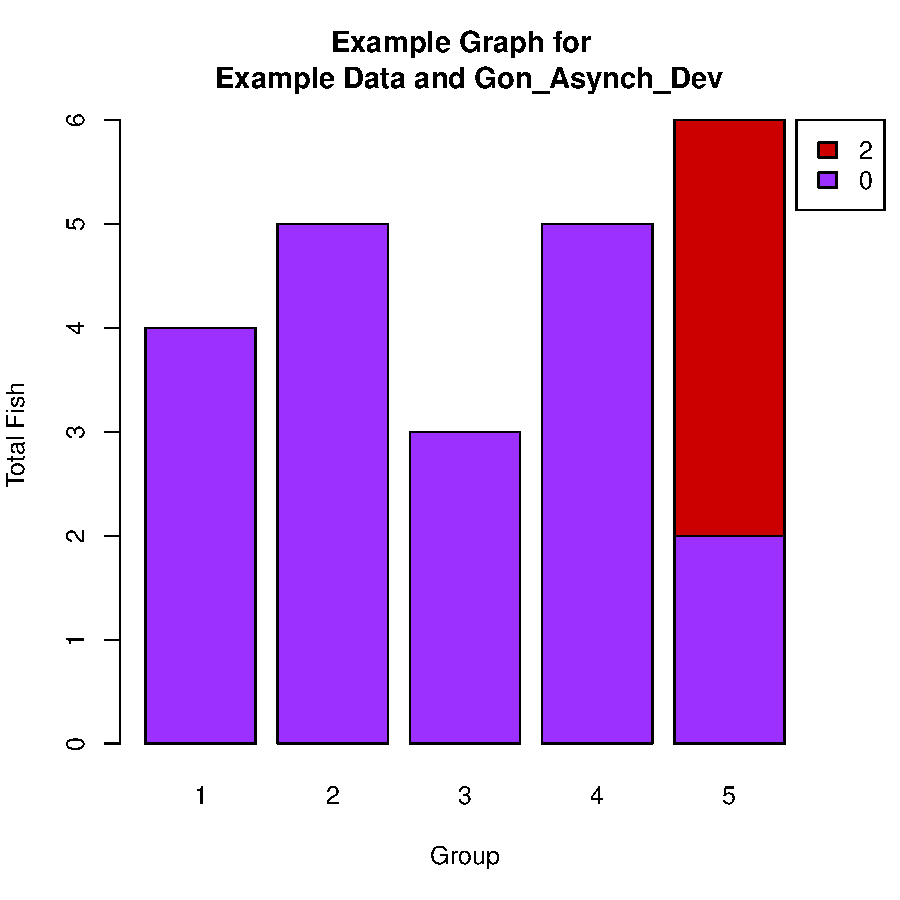
\includegraphics{RSCABS-001}
\end{center}


The arguments of the function are; \textbf{Data}, which 
is \hyperref[subsec:Data]{a standard data set used by RSCABS}, \textbf{Effect} which is 
the name of the endpoint plotted, and \textbf{Treatment} which is the name
of the treatment variable.  \hyperlink{here:metric}{\textbf{Metric}} controls for plotting either total counts ("Total") 
or percent of total counts ("Percent"), while 
\textbf{Lowest} allows for the removal ("Remove") or inclusion ("Include") of non-effected responses. \textbf{Format} is the name of any 
\hyperlink{fig:PlottingFormates}{file format} R can save graphs in, including high resolution graphs which are saved using the 'tiff' format. \textbf{File} is the name of the file the graph is saved to. 
Lastly, the \textbf{plotRSCABS} function can also include any argument used by the \textbf{barplot} function.              




\section*{References}
\label{sec:References}
\thispagestyle{plain}
\addcontentsline{toc}{section}{References}	

[1] Armitage, P. 1955. Tests for Linear Trends in Proportions and Frequencies. \textit{Biometrics} \textbf{11}(3): 417\textemdash451

[2] Cochran, WG 1954. Some methods for strengthening the common chi-squared tests. \textit{Biometrics}  \textbf{10}(4): 417\textemdash451

[3] Green, John W. and Springer, Timothy A. and Saulnier, Amy N. and Swintek, Joe. 2014 Statistical analysis of histopathological endpoints. 
\textit{Environmental Toxicology and Chemistry}, \textbf{33}(5): 1108\textemdash1116

[4] OECD Guidelines for the Testing of Chemicals, Section 2. Test No. 240. DOI10.1787/20745761 

[5] Rao, J. N. K. & Scott, A. J. A. 1992. Simple Method for the Analysis of Clustered Data. \textit{Biometrics}, \textbf{48}: 577\textemdash586. 




\end{document}

















